\documentclass[xcolor=dvipsnames]{beamer}
\usepackage{lmodern}
\usepackage[T1]{fontenc}
\usepackage[english]{babel}
\usepackage[utf8]{inputenc}

\usepackage{manfnt}
\usepackage{wasysym}
\usepackage{listings}
\usepackage{graphicx}
\usepackage{url}
\usepackage{ulem}
\usepackage{marvosym}
\usepackage{skull}
\usepackage{proof}
\usepackage{array}
\usepackage{colortbl}
\setbeamertemplate{navigation symbols}{}

\title[Landslide]{{\bf Landslide: A New Race-Finding Tool for 15-410}}
\subtitle[]{ {\em more clever than } ``\texttt{mandelbrot}'' {\em since 2011.}}
\author[Ben Blum]{Ben Blum \texttt{(bblum@andrew.cmu.edu)}}

\institute[CMU 15-410]{Carnegie Mellon University - 15-410}
\date[]{2016, February 10}

\setbeamertemplate{footline}{\hspace*{.5cm}\scriptsize{\insertauthor\hspace*{50pt} \hfill\insertframenumber\hspace*{.5cm}}} 

\usecolortheme{seahorse}
\usecolortheme{rose}
\useoutertheme{infolines}

\usecolortheme[named=ForestGreen]{structure}

\newcommand\noob{\mathsf{noob}}
\newcommand\gibs{\mathsf{gibs}}
\newcommand\dps{\mathsf{dps}}
\newcommand\squig\rightsquigarrow
\newcommand\Coloneqq{\mathrel{\mathop{::}}=}
\newcommand\dmg{\text{\Laserbeam}}
\newcommand\delter\delta
\newcommand\alpher\alpha
\newcommand\defnor{\text{ }|\text{ }}

\newcommand\pimp{\mathop{\supset}}
\newcommand\pand{\mathop{\wedge}}
\newcommand\por{\mathop{\vee}}
\newcommand\ptrue{\top}
\newcommand\pfalse{\bot}

\newcommand\hilight[2]{\color{#1}#2\color{black}}
\definecolor{olivegreen}{RGB}{0,127,0}

\begin{document}
\renewcommand{\inserttotalframenumber}{39}
\normalem
\begin{frame}
	\titlepage
\end{frame}

%%%%%%%%%%%%%%%%%%%%%%%%%%%%%%%%%%%%%%%%%%%%%%%%%%%%%%%%%%%%%%%%%%%%%%%%%%%%%%%%
%%%%%%%%%%%%%%%%%%%%%%%%%%%%%%%%%%%%%%%%%%%%%%%%%%%%%%%%%%%%%%%%%%%%%%%%%%%%%%%%
%%%%%%%%%%%%%%%%%%%%%%%%%%%%%%%%%%%%%%%%%%%%%%%%%%%%%%%%%%%%%%%%%%%%%%%%%%%%%%%%

\newcommand\linegap{\vspace{0.2in}}
\newcommand\breakslide[1]{\begin{frame}{} \begin{center} #1 \end{center} \end{frame}}

\section{Introduction}
\subsection{Introduction}

\begin{frame}{Outline}
	\textbf{Theory: Seeing race conditions in a new way}
	\begin{itemize}
		\item Case study (example)
		\item Tabular execution traces
		\item The execution tree
	\end{itemize}
	{\bf Research Technique: ``Systematic testing''}
	% Say: A way of enumerating all possible interleavings of a concurrent test case.
	\begin{itemize}
		\item Preemption points
		\item Challenges and feasibility
	\end{itemize}
	{\bf Tool: Landslide}
	\begin{itemize}
		\item How it works
		\item Automatically choosing preemption points
		\item User study (that's you!)
			% !!! SAY !!! : If you are struggling, this is not for you, etc.
	\end{itemize}
\end{frame}

\subsection{Race Conditions}

\definecolor{thread1}{RGB}{87,172,255}
\definecolor{thread2}{RGB}{255,201,102}
\definecolor{thread3}{RGB}{255,128,160}

\begin{frame}{Case Study}
	\begin{center}
		\begin{tabular}{llll}
			\fbox{
			\begin{tabular}{l}
				Consumer thread \\
				\hline
				\\
				\texttt{mutex\_lock(mx);} \\
				\\
				\texttt{if~(!work\_exists())} \\
				\texttt{~~~~cond\_wait(cvar,~mx);} \\
				\texttt{work~=~dequeue();} \\
				\\
				\texttt{mutex\_unlock(mx);} \\
				\texttt{access(work->data);} \\
			\end{tabular}
			}
			& & &
			\fbox{
			\begin{tabular}{l}
				Producer thread \\
				\hline
				\\
				\texttt{mutex\_lock(mx);} \\
				\\
				\texttt{enqueue(work);} \\
				\texttt{signal(cvar);} \\
				\\
				\texttt{mutex\_unlock(mx);} \\
				\\
				\\
			\end{tabular}
			}
		\end{tabular}
		\linegap

		\begin{itemize}
			\item See {\bf Paradise Lost} lecture!
			\item {\tt if} vs {\tt while}: Two consumers can race to make one fail.
		\end{itemize}
	\end{center}
\end{frame}
\begin{frame}{Thread Interleavings (``good'' case)}
	\begin{center}
		\begin{tabular}{|l|l|l|}
			\hline
			\cellcolor{thread1} {\bf Thread 1} & \cellcolor{thread2} {\bf Thread 2} & \cellcolor{thread3} {\bf Thread 3} \\
			\hline
			\small \texttt{lock(mx);} & & \\
			\small \texttt{if~(!work\_exists())} & & \\
			\small \texttt{~~~~wait(cvar,~mx);} & & \\
			
			& & \small \texttt{lock(mx);} \\
			& & \small \texttt{if~(!work\_exists())} \\
			& & \small \texttt{~~~~wait(cvar,~mx);} \\

			& \small \texttt{lock(mx);} & \\
			& \small \texttt{enqueue(work);} & \\
			& \small \texttt{signal(cvar);} & \\
			& \small \texttt{unlock(mx);} & \\
			
			\small \texttt{work~=~dequeue();~} & & \\
			\small \texttt{unlock(mx);} & & \\
			\small \texttt{access(work->data);}& & \\
			\hline
		\end{tabular}
	\end{center}
\end{frame}
\begin{frame}{Thread Interleavings (different ``good'' case)}
	\begin{center}
		\begin{tabular}{|l|l|l|}
			\hline
			\cellcolor{thread1} {\bf Thread 1} & \cellcolor{thread2} {\bf Thread 2} & \cellcolor{thread3} {\bf Thread 3} \\
			\hline
			\small \texttt{lock(mx);} & & \\
			\small \texttt{if~(!work\_exists())} & & \\
			\small \texttt{~~~~wait(cvar,~mx);} & & \\
			
			& \small \texttt{lock(mx);} & \\
			& \small \texttt{enqueue(work);} & \\
			& \small \texttt{signal(cvar);} & \\
			& \small \texttt{unlock(mx);} & \\
			
			\small \texttt{work~=~dequeue();~} & & \\
			\small \texttt{unlock(mx);} & & \\
			\small \texttt{access(work->data);}& & \\
			
			& & \small \texttt{lock(mx);} \\
			& & \small \texttt{if~(!work\_exists())} \\
			& & \small \texttt{~~~~wait(cvar,~mx);} \\
			\hline
		\end{tabular}
	\end{center}
\end{frame}
\begin{frame}{Thread Interleavings (race condition)}
	\begin{center}
		\begin{tabular}{|l|l|l|}
			\hline
			\cellcolor{thread1} {\bf Thread 1} & \cellcolor{thread2} {\bf Thread 2} & \cellcolor{thread3} {\bf Thread 3} \\
			\hline
			\small \texttt{lock(mx);} & & \\
			\small \texttt{if~(!work\_exists())} & & \\
			\small \texttt{~~~~wait(cvar,~mx);} & & \\
			
			& \small \texttt{lock(mx);} & \\
			& \small \texttt{enqueue(work);} & \\
			& \small \texttt{signal(cvar);} & \\
			& \small \texttt{unlock(mx);} & \\
			
			& & \small \texttt{lock(mx);} \\
			& & \small \texttt{work~=~dequeue();~~} \\
			& & \small \texttt{unlock(mx);} \\

			\small \texttt{work~=~dequeue();} & & \\
			\small \texttt{unlock(mx);} & & \\
			\small \texttt{//~SIGSEGV} {\large \frownie}& & \\
			\hline
		\end{tabular}
	\end{center}
\end{frame}


\begin{frame}{Testing}
	How can programmers be confident in the correctness of their code?
	\begin{itemize}
		\item Unit tests
		\begin{itemize}
			\item good for basic functionality, bad for concurrency
		\end{itemize}
		\item Stress tests
		\begin{itemize}
			\item state of the art in 15-410
		\end{itemize}
		\item Theorem proving
		\begin{itemize}
			\item heavy burden on the programmers
		\end{itemize}
		\item Releasing to paying customers and worrying about correctness later
			% Say... "and I'm hoping to prevent you from finding yourself in a future where this happens!"
	\end{itemize}
	\linegap

	{\bf Motivation}: Can we do better than stress testing?
\end{frame}

\begin{frame}{Testing Mechanisms}
	\textbf{Stress testing}: \texttt{largetest}, \texttt{mandelbrot} and friends
	\begin{itemize}
		\item Attempting to exercise as many interleavings as practical
		\item Exposes race conditions at random
		\begin{itemize}
			\item ``If a preemption occurs at just the right time\ldots''
		\end{itemize}
		\item Cryptic panic messages when failure occurs
	\end{itemize}
	\linegap
	What if\ldots
	\begin{itemize}
		\item Make educated guesses about when to preempt
		\item Preempt enough times to run {\em every single} interleaving
		\item Tell the story of what {\em actually happened}.
		\item Overlook fewer bugs!
	\end{itemize}
	% Say: At the end of this lecture, I'm going to be looking for some among you...
\end{frame}

%%%%%%%%%%%%%%%%%%%%%%%%%%%%%%%%%%%%%%%%%%%%%%%%%%%%%%%%%%%%%%%%%%%%%%%%%%%%%%%%
%%%%%%%%%%%%%%%%%%%%%%%%%%%%%%%%%%%%%%%%%%%%%%%%%%%%%%%%%%%%%%%%%%%%%%%%%%%%%%%%
%%%%%%%%%%%%%%%%%%%%%%%%%%%%%%%%%%%%%%%%%%%%%%%%%%%%%%%%%%%%%%%%%%%%%%%%%%%%%%%%

\section{Systematic Testing}

\breakslide{\Large A different way of looking at race conditions\ldots}

\begin{frame}{Execution Tree}
		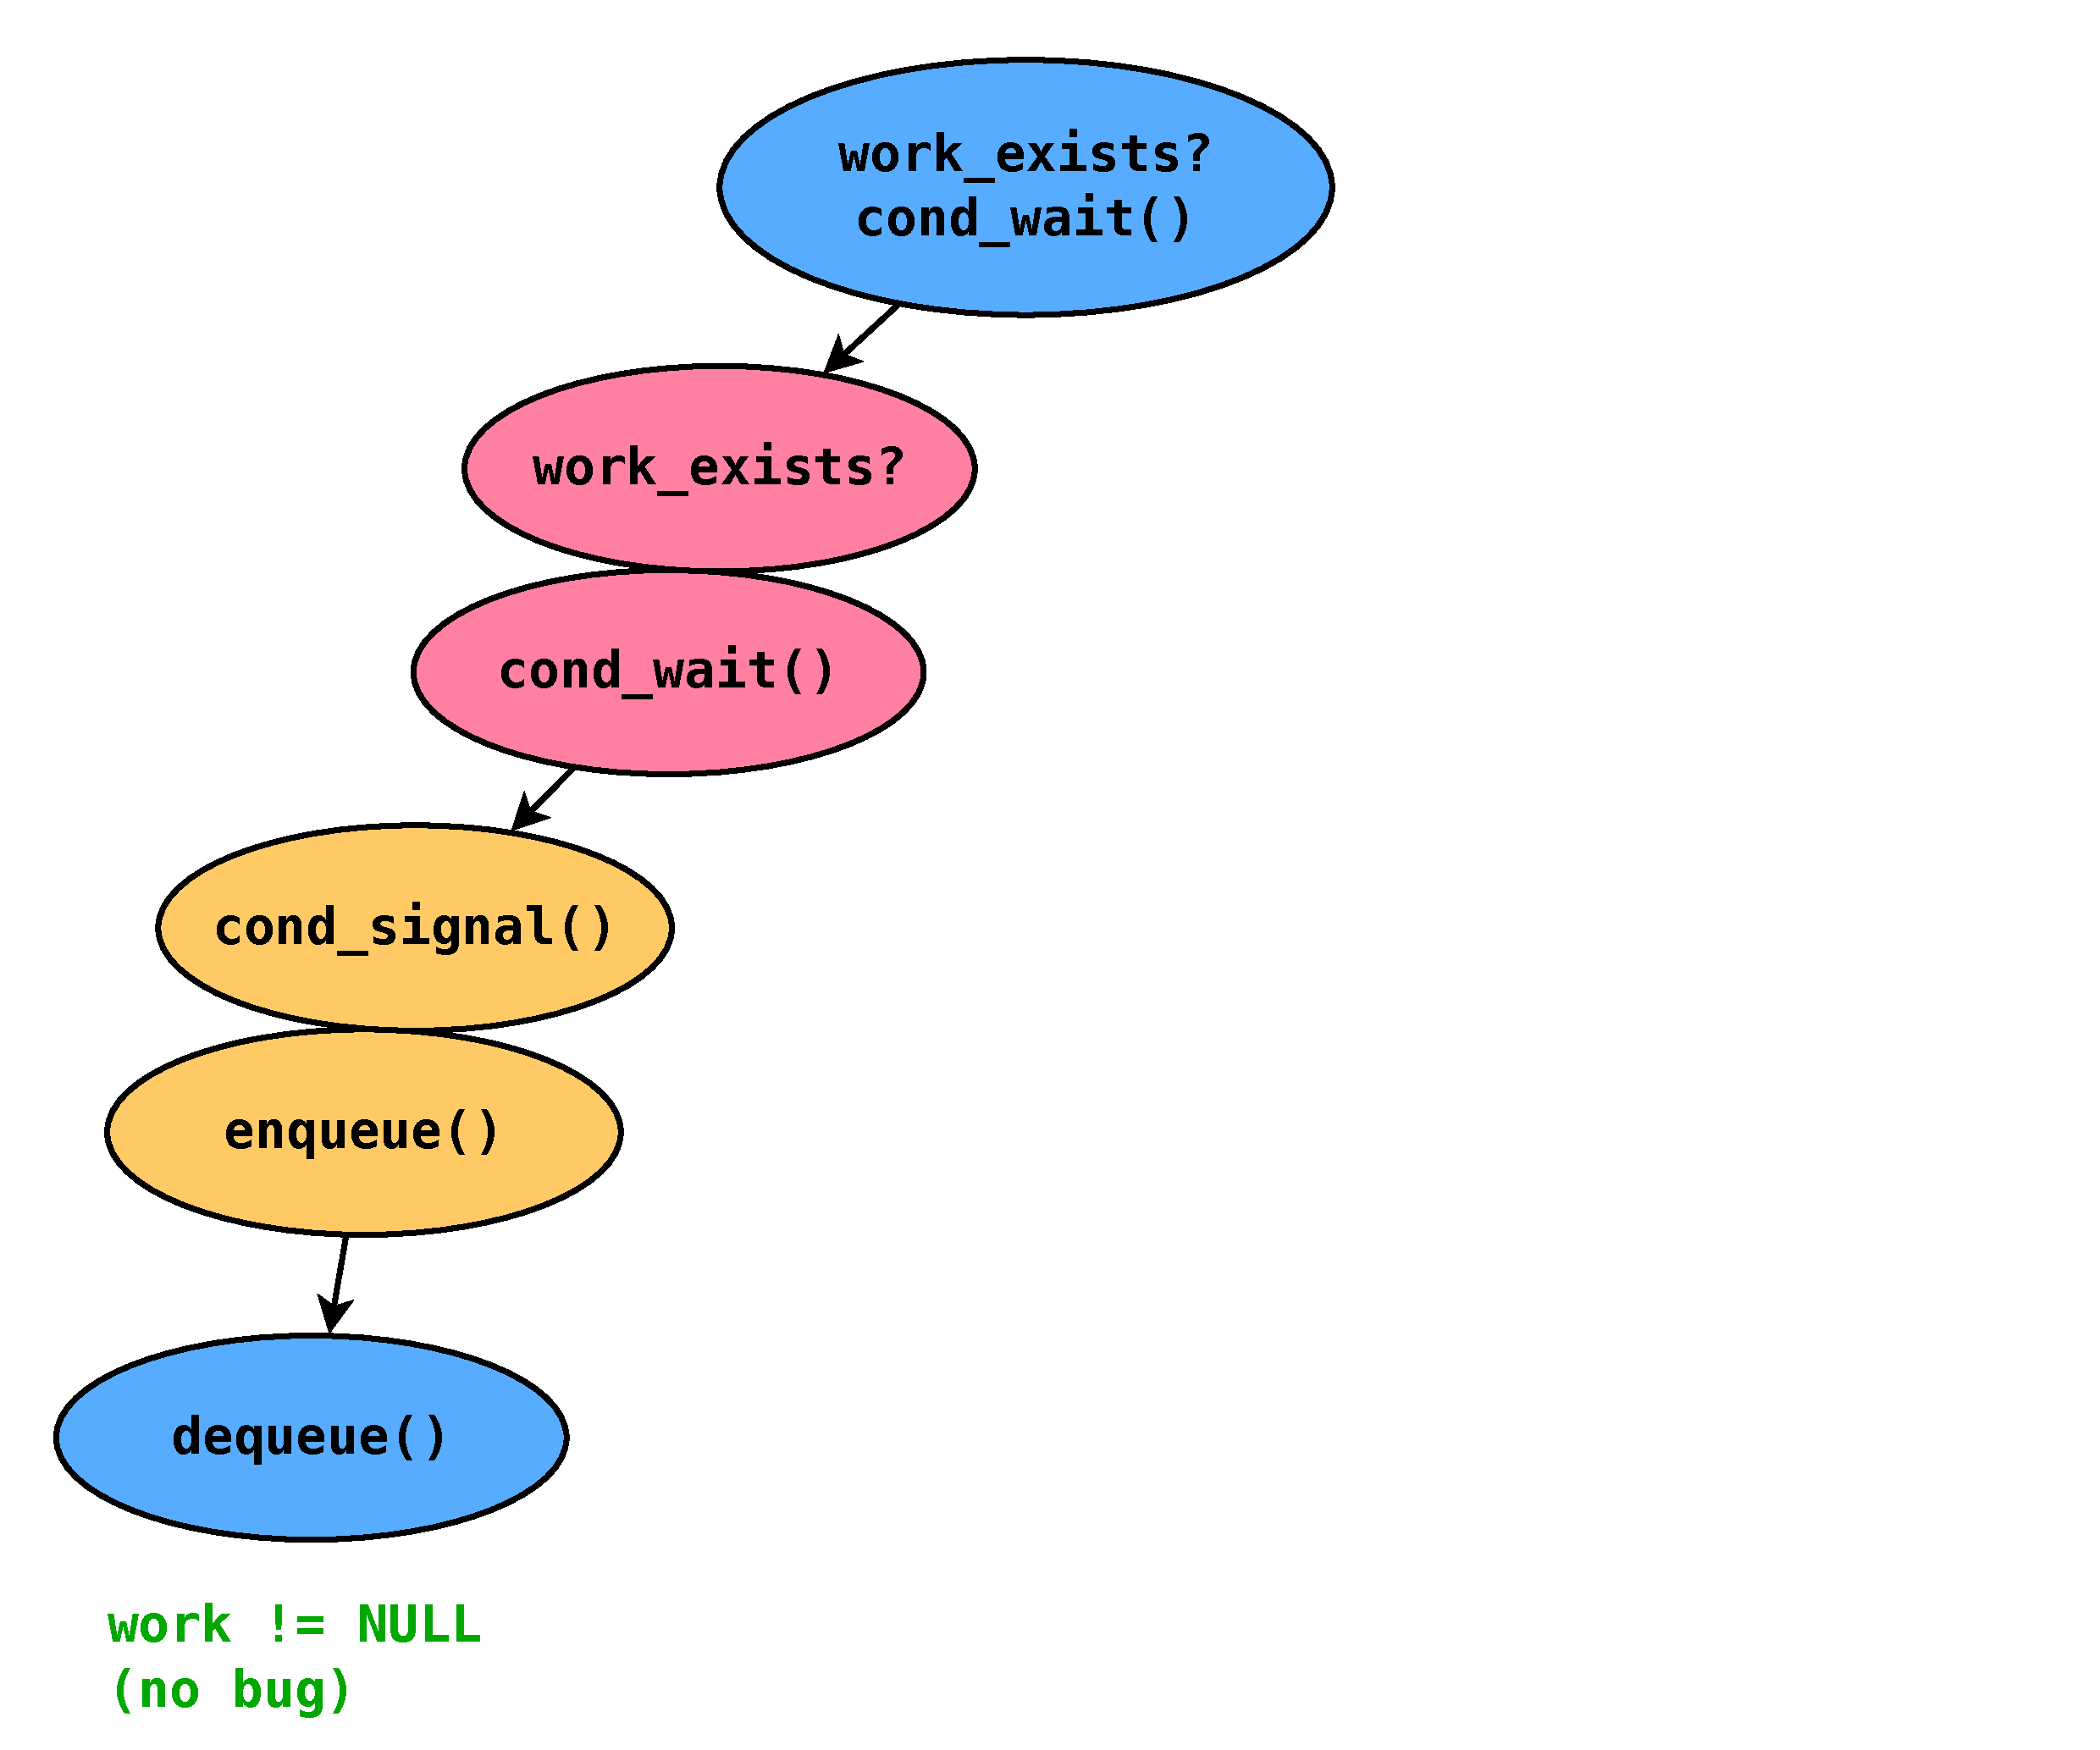
\includegraphics[width=0.78\textwidth]{execution-tree-0.pdf} \\
		\vspace{-3in}
		\hspace{3in}
		\includegraphics[width=0.34\textwidth]{table-0.png}
		\\
		\vspace{1.2in}
		\hspace{3.7in}
		
\includegraphics[width=0.15\textwidth]{frownie-blank.png}
\end{frame}
\begin{frame}{Execution Tree}
		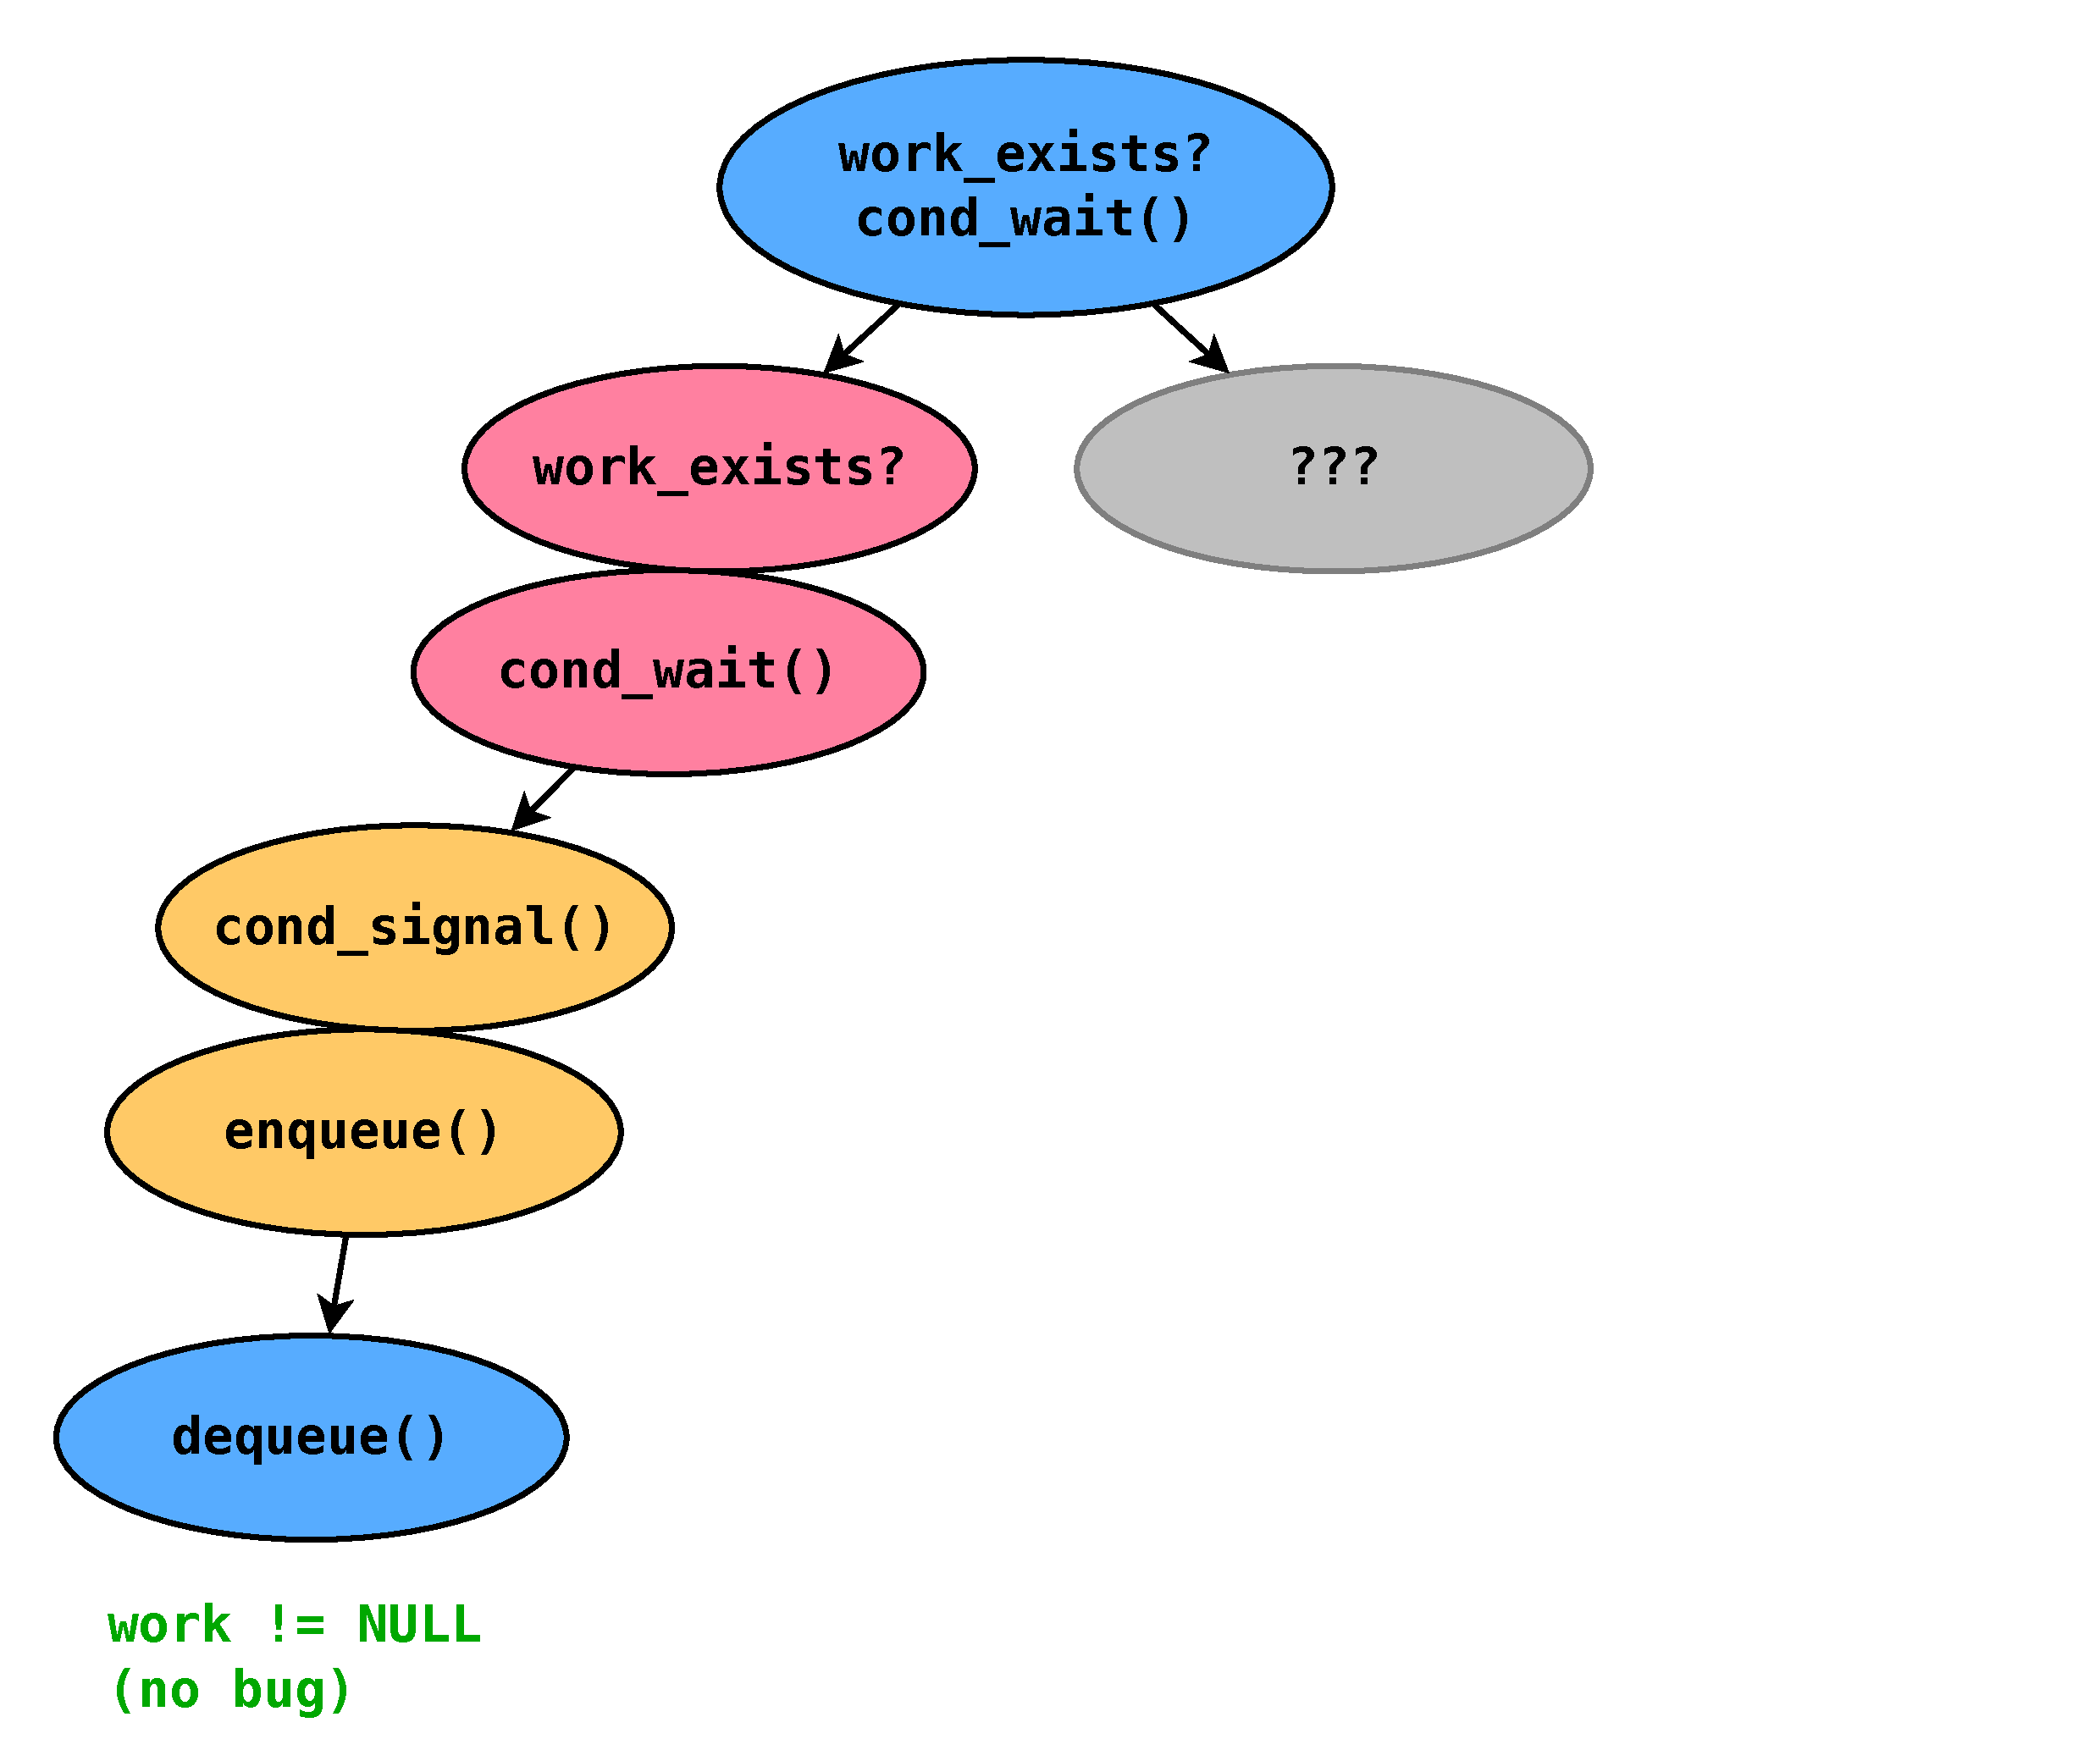
\includegraphics[width=0.78\textwidth]{execution-tree-1.pdf} \\
		\vspace{-3in}
		\hspace{3in}
		\includegraphics[width=0.34\textwidth]{table-0.png}
		\\
		\vspace{1.2in}
		\hspace{3.7in}
		
\includegraphics[width=0.15\textwidth]{frownie-blank.png}
\end{frame}
\begin{frame}{Execution Tree}
		\includegraphics[width=0.78\textwidth]{execution-tree-2.pdf} \\
		\vspace{-3in}
		\hspace{3in}
		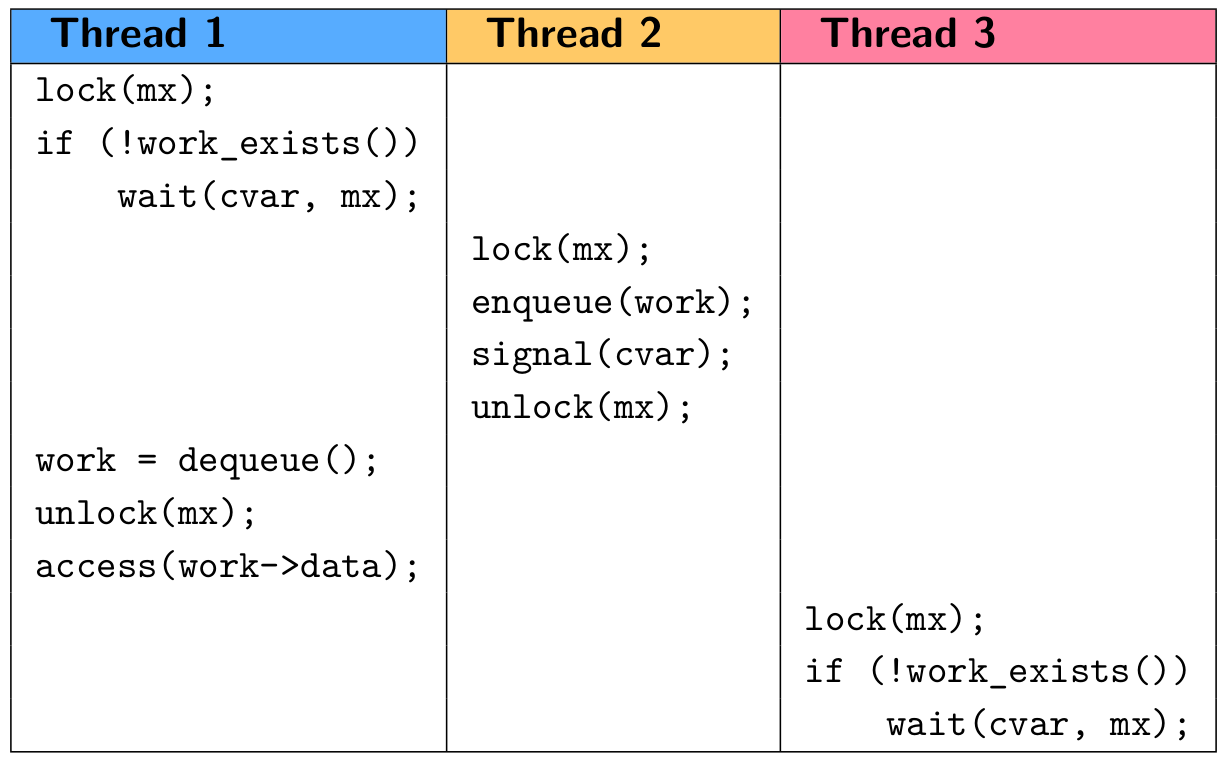
\includegraphics[width=0.34\textwidth]{table-1.png}
		\\
		\vspace{1.2in}
		\hspace{3.7in}
		
\includegraphics[width=0.15\textwidth]{frownie-blank.png}
\end{frame}
\begin{frame}{Execution Tree}
		\includegraphics[width=0.78\textwidth]{execution-tree-full.pdf} \\
		\vspace{-3in}
		\hspace{3in}
		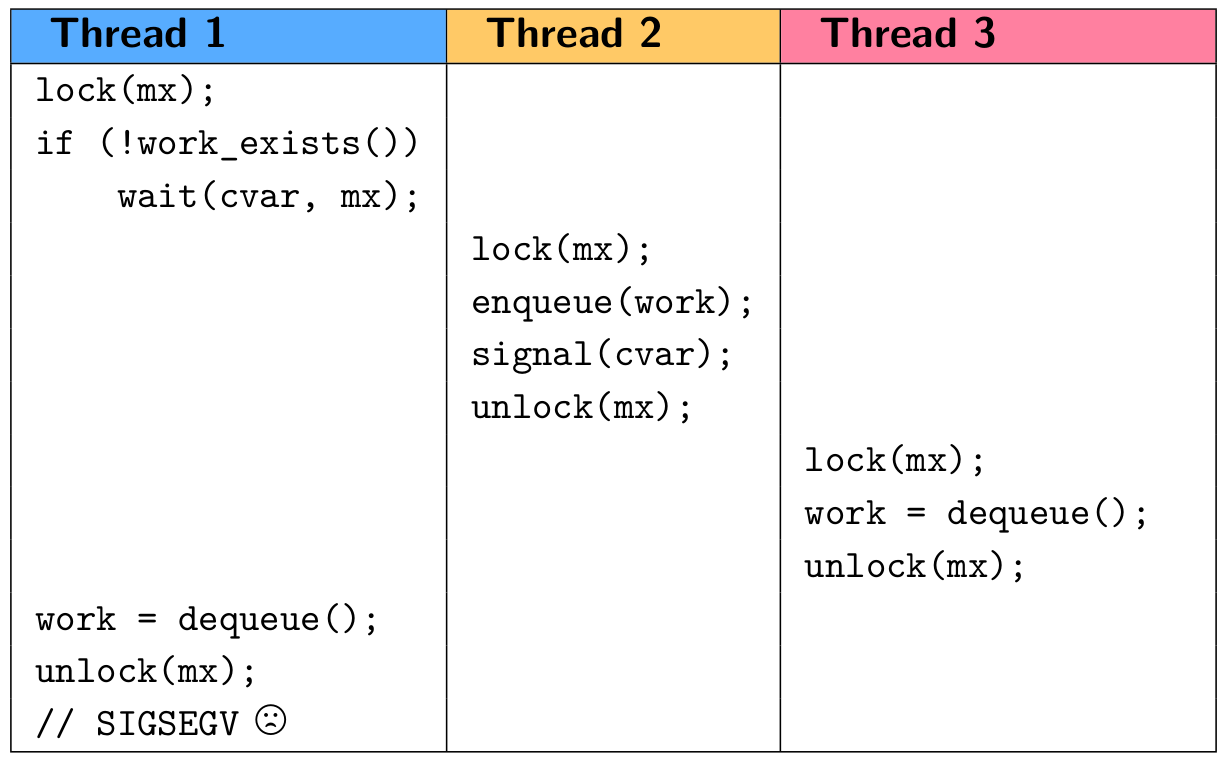
\includegraphics[width=0.34\textwidth]{table-2.png}
		\\
		\vspace{1.2in}
		\hspace{3.7in}
		
\includegraphics[width=0.15\textwidth]{frownie.png}
\end{frame}

% Say: Obviously we want to be able to always run the third path. But knowing
% that ahead of time is impossible.

% Say: In the rest of the lecture I'm going to refer to the "state space of
% possible interleavings", simply referring to this tree, and "size" of the state
% space refers to the number of branches.

\begin{frame}{Systematic Testing - The Big Picture}
	\textbf{Goal: Force the system to execute every possible interleaving.}
	% Say: checking for crashes/memory errors/etc in each one.
	\begin{itemize}
		\item On 1st execution, schedule threads arbitrarily until program ends.
			\begin{itemize}
				\item This represents one branch of the tree.
			\end{itemize}
		\item At end of each branch, rewind system and restart test.
		\item Artificially add preemptions to produce different thread interleavings.
		\item Intuitively: Generate many ``tabular execution traces''.
	\end{itemize}
	\pause
	\linegap

	Okay, wait a sec...
	\begin{itemize}
		\item How can you possibly execute {\em every possible} interleaving?
		%\item How can you know where preempting matters most?
		\item How did you know to draw that tree's branches where they matter?
	\end{itemize}
\end{frame}

\begin{frame}{Preemption Points}
	\textbf{Preemption points} (PPs) are code locations where being preempted may cause different behaviour.
	\begin{itemize}
		\item IOW, somewhere that interesting interleavings can happen around.
	\end{itemize}
	\linegap

	Systematic tests are {\em parameterized} by the set of PPs.
	\begin{itemize}
		\item If there are $n$ PPs and $k$ threads, state space size is $n^k$.
		\item Need to choose the set of PPs very carefully for test to be effective.
		\begin{itemize}
			\item ``Effective'' = both comprehensive and feasible.
		\end{itemize}
	\end{itemize}
\end{frame}


\begin{frame}{Preemption Points}
	What does ``all possible interleavings'' actually mean?

	\linegap
	{\bf One extreme}: Preempt at {\em every instruction}
	\begin{itemize}
		\item Good news: Will find every possible race condition.
		\item Bad news: Runtime of test will be impossibly large.
	\end{itemize}
	\linegap

	{\bf Other extreme}: {\em Nothing} is a preemption point
	\begin{itemize}
		\item Good news: Test will finish quickly.
		\item Bad news: Only one execution was checked for bugginess.
		\begin{itemize}
			\item No alternative interleavings explored.
			\item Makes ``no race found'' a weak claim.
		\end{itemize}
	\end{itemize}
\end{frame}

\begin{frame}{Preemption Point Example (remember this?)}
	\fbox{
	\begin{tabular}{l}
	\texttt{boolean~want[2]~=~\{~false,~false~\};}\\
	\\
	\begin{tabular}{rll}
		1 & \texttt{want[i]~=~true;} & \\
		  & & \footnotesize (preemption point A) \\
		2 & \texttt{while~(want[j])} & \\
		  & & \footnotesize (preemption point B) \\
		3 & \texttt{~~~~~~~~continue;} & \\
		  & & \footnotesize (preemption point C) \\
		4 & \texttt{//~...critical~section...} & \\
		  & & \footnotesize (preemption point D) \\
		5 & \texttt{want[i]~=~false;} & \\
	\end{tabular}
	\end{tabular}
	}
	\linegap

	{\bf Some preemption points will expose bugs. \\
	Some preemption points don't matter.}

\end{frame}

\begin{frame}{Preemption Point Example (remember this?)}
	\fbox{
	\begin{tabular}{l}
	\texttt{boolean~want[2]~=~\{~false,~false~\};}\\
	\\
	\begin{tabular}{rll}
		1 & \texttt{want[i]~=~true;} & \\
		  & & \footnotesize (preemption point A) \\
		2 & \texttt{while~(want[j])} & \\
		  & & \footnotesize ~ \\
		3 & \texttt{~~~~~~~~continue;} & \\
		  & & \footnotesize ~ \\
		4 & \texttt{//~...critical~section...} & \\
		  & & \footnotesize ~ \\
		5 & \texttt{want[i]~=~false;} & \\
	\end{tabular}
	\end{tabular}
	}
	\linegap

	Here, only preemption point A will trigger a deadlock. {\bf ~}\\
	All other interleavings are benign.{\bf ~}

\end{frame}

\begin{frame}{Preemption Points}
	\textbf{Sweet spot}: Insert a thread switch everywhere it ``might matter''.

	\linegap
	When do we fear being preempted?
	\begin{itemize}
		\item Threads becoming runnable (\texttt{thr\_create()}, \texttt{cond\_signal()}, etc.)
			\begin{itemize}
				\item Preemptions may cause it to run before we're ready
			\end{itemize}
		\item Synchronization primitives (\texttt{mutex\_lock()}/\texttt{unlock()}, etc.)
			\begin{itemize}
				\item If buggy or used improperly\ldots
			\end{itemize}
		\item Unprotected shared memory accesses (``data races'')% Say: more on this later.
			\begin{itemize}
				\item May result in data structure corruption
				\item More on this later...
			\end{itemize}
	\end{itemize}

	%%%% Not anymore! :D
	%Finding the sweet spot is a joint effort between programmer and tool. (More on this later.)
	%However, all these points together may still be too expensive...
\end{frame}

%\begin{frame}{Challenges}
%	Parameters of systematic tests must be kept small.
%	\begin{itemize}
%		\item Test program length / number of threads
%		\item Number of preemption points used
%	\end{itemize}
%	\linegap
%
%	\begin{center}
%		\hspace{-0.25in}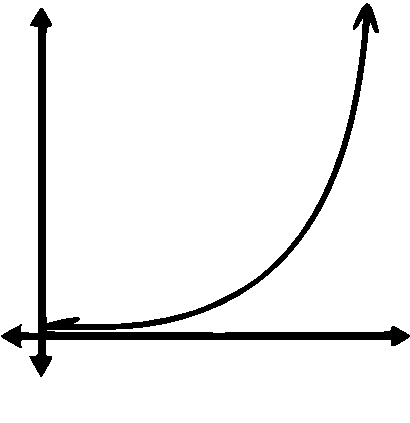
\includegraphics[width=0.3\textwidth]{expo.pdf} \\
%		\vspace{-1.33in}\hspace{-1.75in}{\rotatebox{90}{\small state space size}} \\
%		\vspace{0.15in}\hspace{-0.25in}{\small number of PPs}
%	\end{center}
%\end{frame}

%%%%%%%%%%%%%%%%%%%%%%%%%%%%%%%%%%%%%%%%%%%%%%%%%%%%%%%%%%%%%%%%%%%%%%%%%%%%%%%%
%%%%%%%%%%%%%%%%%%%%%%%%%%%%%%%%%%%%%%%%%%%%%%%%%%%%%%%%%%%%%%%%%%%%%%%%%%%%%%%%
%%%%%%%%%%%%%%%%%%%%%%%%%%%%%%%%%%%%%%%%%%%%%%%%%%%%%%%%%%%%%%%%%%%%%%%%%%%%%%%%

\section{Landslide}

\breakslide{\Huge Landslide}

\begin{frame}{About The Project}
	\textbf{About me}: 5th year graduate student, advised by Garth Gibson
	\begin{itemize}
		\item TAed 15-410 for 3 semesters during undergrad
		\item 1st graduate year was 5th year M.S., rest in Ph.D. program
		\begin{itemize}
			\item \url{http://www.contrib.andrew.cmu.edu/~bblum/thesis.pdf}
		\end{itemize}
	\end{itemize}
	\pause
	\linegap

	{\bf About Landslide}
	\begin{itemize}
		\item Simics module, which traces:
			\begin{itemize}
				\item Every instruction executed
				\item Every memory access read/written
			\end{itemize}
			% FIXME for next year -- how much slowdown is there? 20x?
		\item Originally supported only P3s; can now test P2s fully-automated
		\item {\em Landslide} shows how your {\em Pebbles} programs may not be stable.
	\end{itemize}
\end{frame}

%%%%%%%%%%%%%%%%%%%%%%%%%%%%%%%%%%%%%%%%%%%%%%%%%%%%%%%%%%%%%%%%%%%%%%%%%%%%%%%%

\subsection{Technical Overview}

\begin{frame}{Big Picture: Execution Tree Exploration}
	\textbf{Backtracking}
	\begin{itemize}
		\item At end of each branch, identify a PP to replay differently
		\item Reset machine state and start over
		\item Implemented using Simics bookmarks
			\begin{itemize}
				\item {\tt set-bookmark} and {\tt skip-to}
			\end{itemize}
		\item Replay test from the beginning, with a different interleaving
	\end{itemize}
	\pause
	\linegap

	{\bf Controlling scheduling decisions}
	\begin{itemize}
		\item Tool must control all sources of nondeterminism
		\item In 15-410, just timer and keyboard interrupts
			% optional - say: "in real kernels, disk/network io interrupts"
		\item Landslide repeatedly fires timer ticks until desired thread is run.
	\end{itemize}
\end{frame}

\begin{frame}{Landslide \& You}
	\begin{center}
	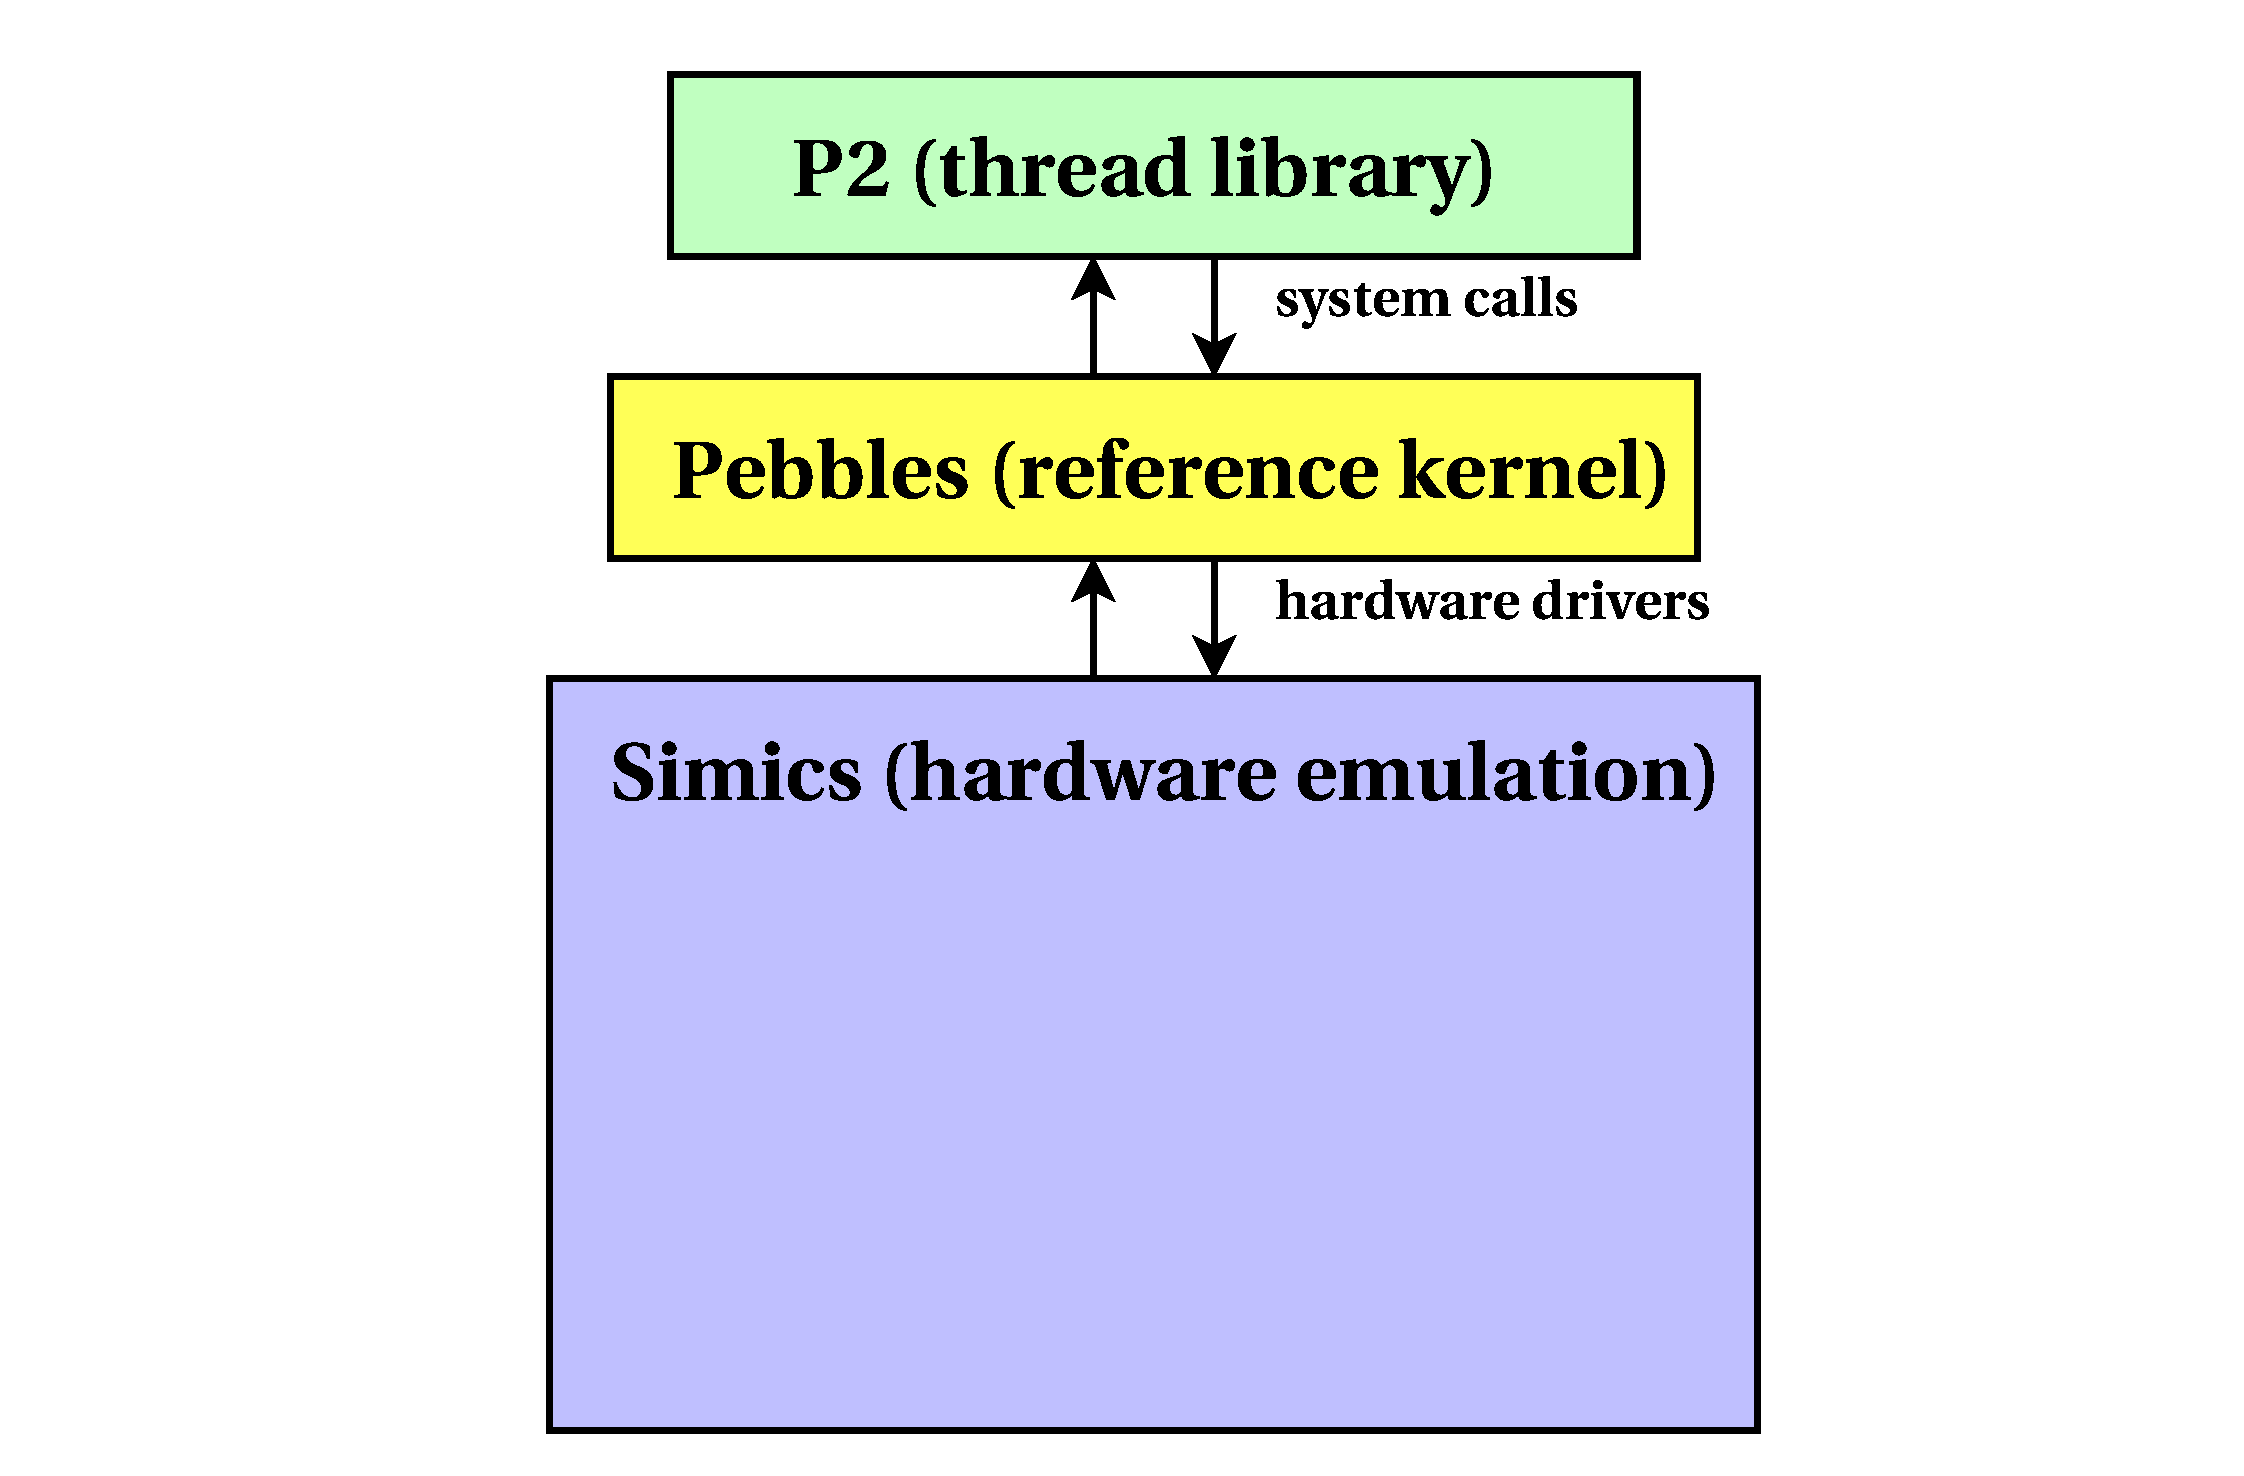
\includegraphics[width=0.85\textwidth]{landslide-new-blank.pdf}
	\end{center}
\end{frame}

\begin{frame}{Landslide \& You}
	\begin{center}
	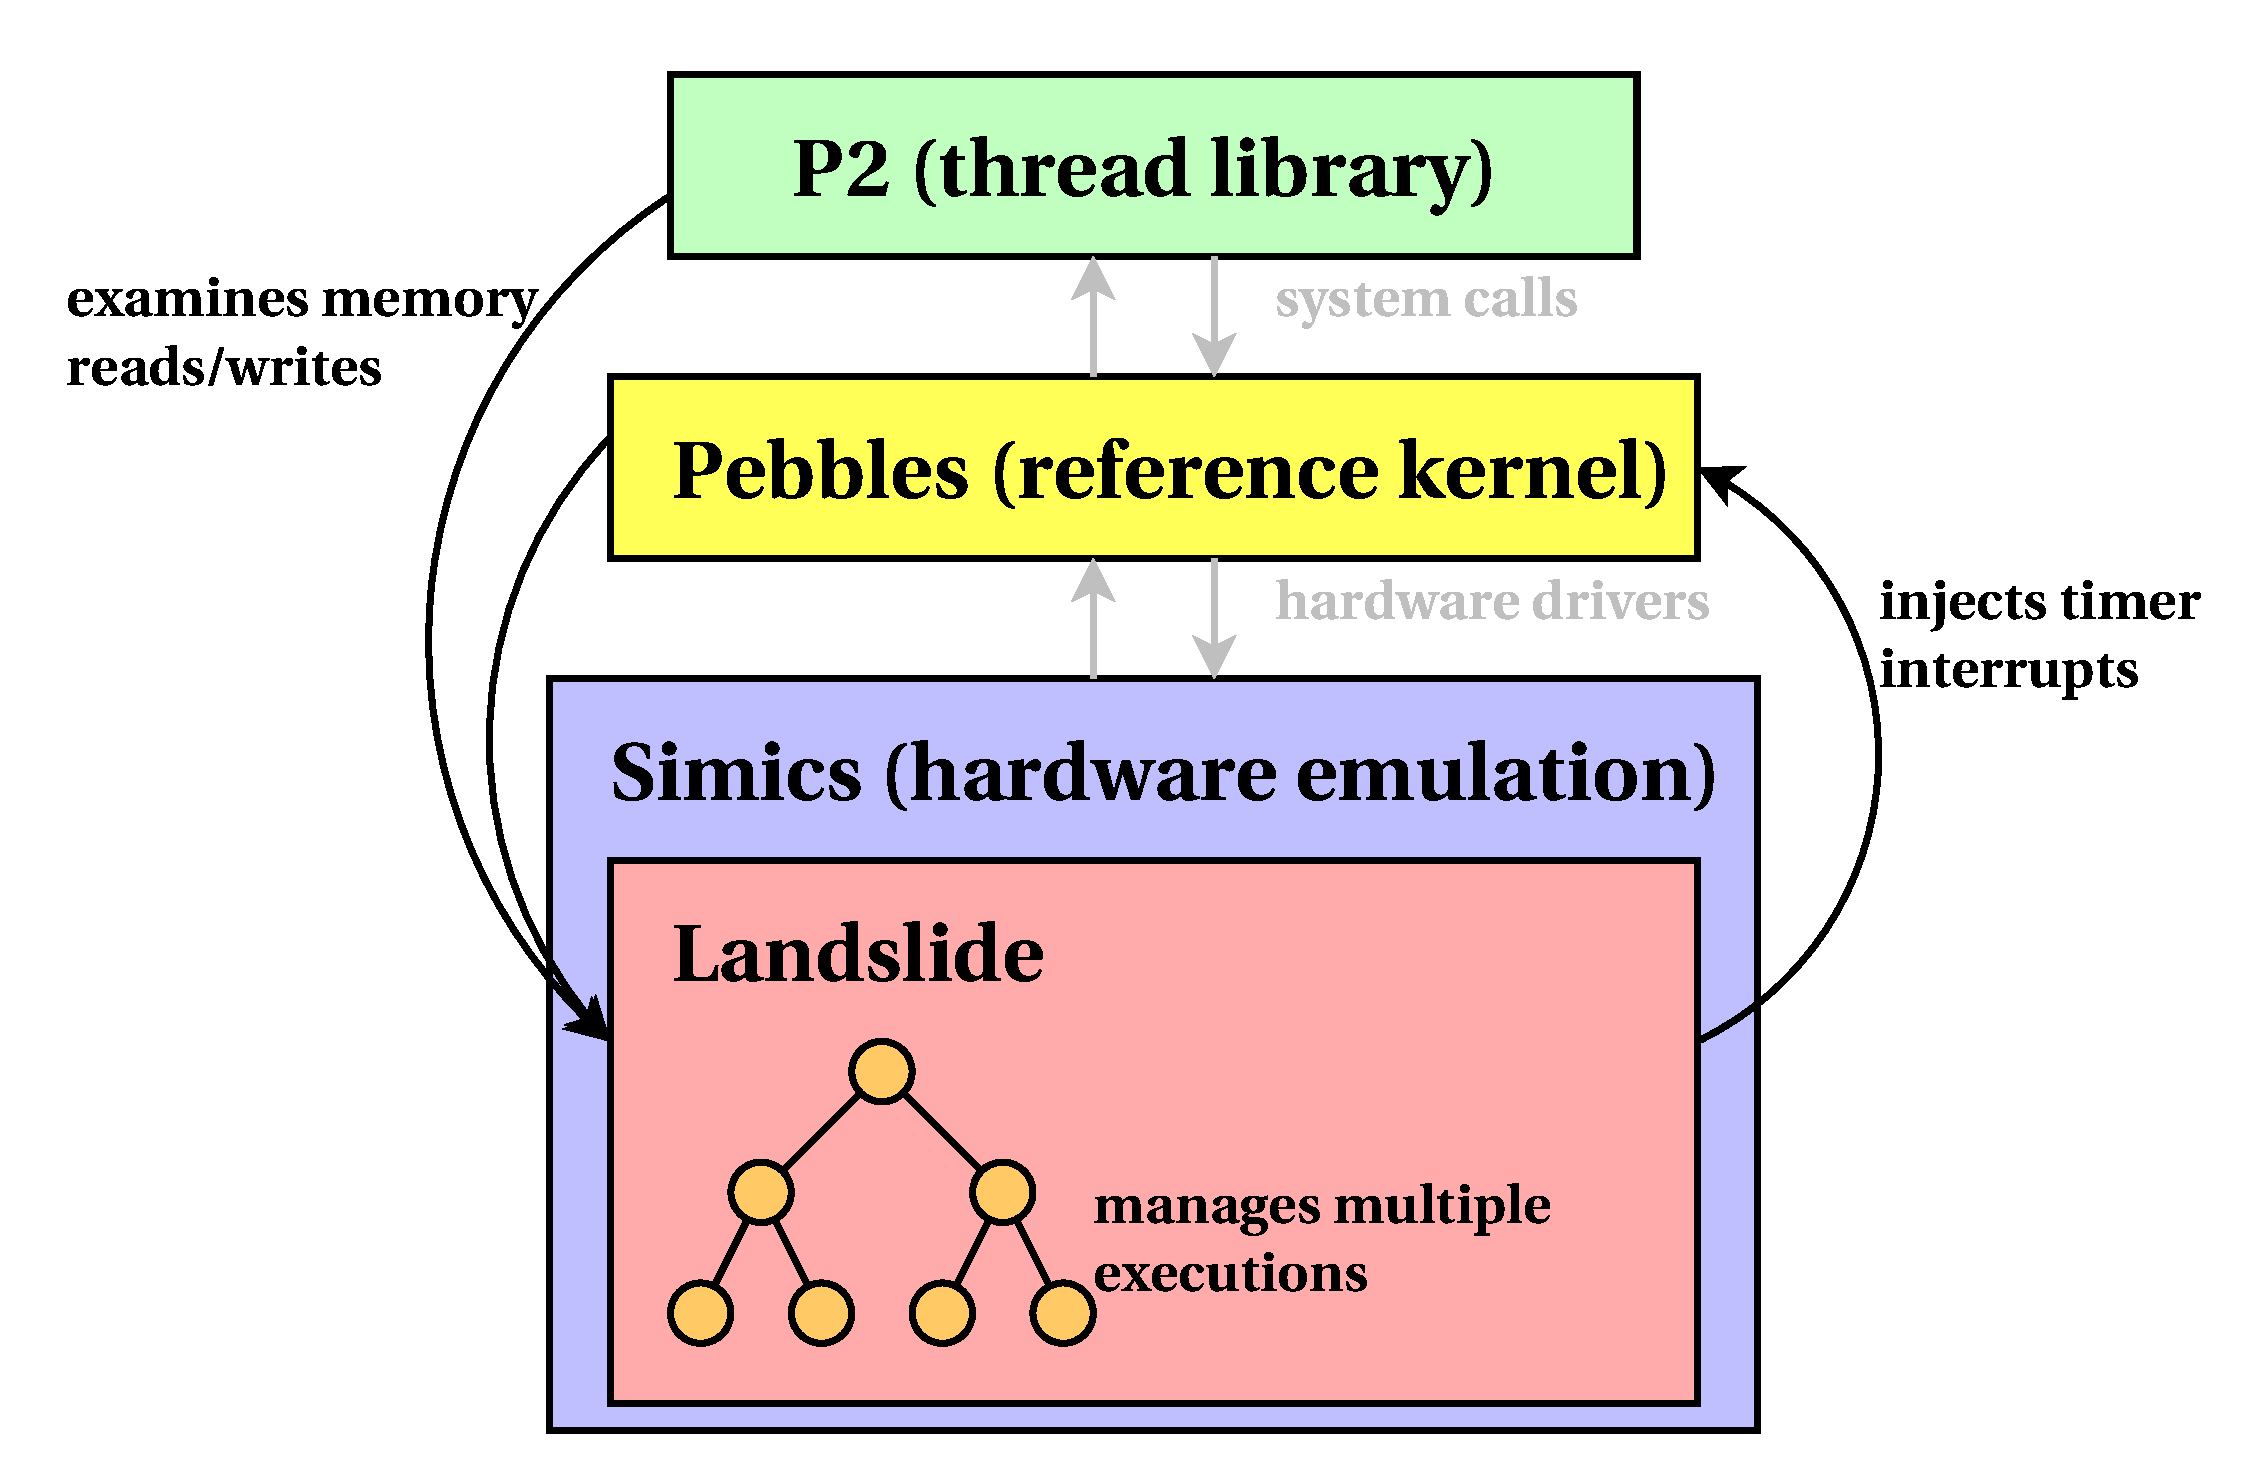
\includegraphics[width=0.85\textwidth]{landslide-new.pdf}
	\end{center}
\end{frame}

\begin{frame}{Identifying Bugs}
	Landslide can {\em definitely discover:}
	\begin{itemize}
		\item Assertion failures % Say: note: the better your asserts are..!
		\item Segfaults
		\item Deadlock
		\item Use-after-free / double-free
	\end{itemize}
	\linegap
	Landslide can {\em reasonably suspect:}
	\begin{itemize}
		\item Infinite loop (halting problem)
		\item Data race bugs
	\end{itemize}
\end{frame}

\begin{frame}{What is a Data Race?}
	A {\bf data race} is a pair of memory accesses between two threads, where:
	\begin{itemize}
		\item At least one of the accesses is a write
		\item The threads are not holding the same mutex
		\item The threads can be reordered (e.g., no \texttt{cond\_signal()} in between)
	\end{itemize}
	\pause
	\linegap

	Data races are {\em not necessarily} bugs, just highly suspicious!
	\begin{itemize}
		\item Bakery alg: Is {\tt number[i]=max(number[0],number[1])+1} bad?
		%\item Is unprotected {\tt foobar\_statistics\_counter++} bad?
		\item What about unprotected {\tt next\_thread\_id++}?
		\item ``If threads interleaved the wrong way here, it {\em might} crash later.''
		\begin{itemize}
			\item Hmmm...
		\end{itemize}
	\end{itemize}
\end{frame}

%%%%%%%%%%%%%%%%%%%%%%%%%%%%%%%%%%%%%%%%%%%%%%%%%%%%%%%%%%%%%%%%%%%%%%%%%%%%%%%%

\subsection{Iterative Deepening}

\begin{frame}{Choosing the Right Preemption Points}
	How can we address exponential state space explosion?
	\pause
	\linegap

	State of the art tools hard-code a fixed set of preemption points.
	\begin{itemize}
		\item E.g., ``all thread library API calls'' or ``all kernel mutex locks/unlocks''
		\item Depending on length of test, completion time is unpredictable.
		\item More often, a subset is better in terms of time/coverage. 
	\end{itemize}
	\pause
	\linegap
	Current systematic testing model is not user-friendly.
	\begin{itemize}
		\item Tool: ``I want to use these PPs, but can't predict completion time.''
		\item User: ``I have 16 CPUs and 24 hours to test my program.''
	\end{itemize}
	\linegap
	{\em Stress testing allows user to choose total run time -- can we offer this too?}
\end{frame}

\begin{frame}{Iterative Deepening of Preemption Points}
	Goal: Run the best tests for a given CPU budget.
	\begin{itemize}
		\item Technique: ``Iterative Deepening''
	\end{itemize}
	\linegap

	Based on experience from past 15-410 student volunteers
	\begin{itemize}
		%\item Students worked best with an iterative process
		\item ``Start small, then add more preemption points as time allows''
		\item Landslide now automates this process
	\end{itemize}
	\linegap

	Named after analogous technique in chess AI.
	\begin{itemize}
		\item Chess search is DFS limited by max number of moves (ply).
		\item Chess AIs repeat DFS, increasing ply, until timeout.
	\end{itemize}
\end{frame}

\begin{frame}{Iterative Deepening in Landslide}
	Landslide automatically iterates through different configurations of PPs.
	\begin{itemize}
		\item Manages work queue of jobs with different PPs
		\item Each job represents a new state space for Landslide to explore
		\item Prioritizes jobs based on estimated completion time
		%\item Prioritizes which jobs are important / likely to finish
		%\begin{itemize}
		%	\item Based on nature of PPs (data races? mutexes?)
		%	\item Based on estimated completion time
		%\end{itemize}
	\end{itemize}
	\linegap

	Repeat state space explorations, adding preemption points, until time is exhausted.

	\linegap
	{\em Only required argument is CPU budget}
\end{frame}

\begin{frame}{Iterative Deepening}
	Minimal state space includes only ``mandatory'' context switches
	\begin{itemize}
		\item e.g., {\tt yield()}, {\tt cond\_wait()}.
		% Say: When the test invokes yield, the kernel scheduler will pick
		% one thread to run next. With Landslide, we will pick ALL threads to
		% run next, in one parallel universe at a time.
	\end{itemize}
	\vspace{0.29in}
	\begin{center}
		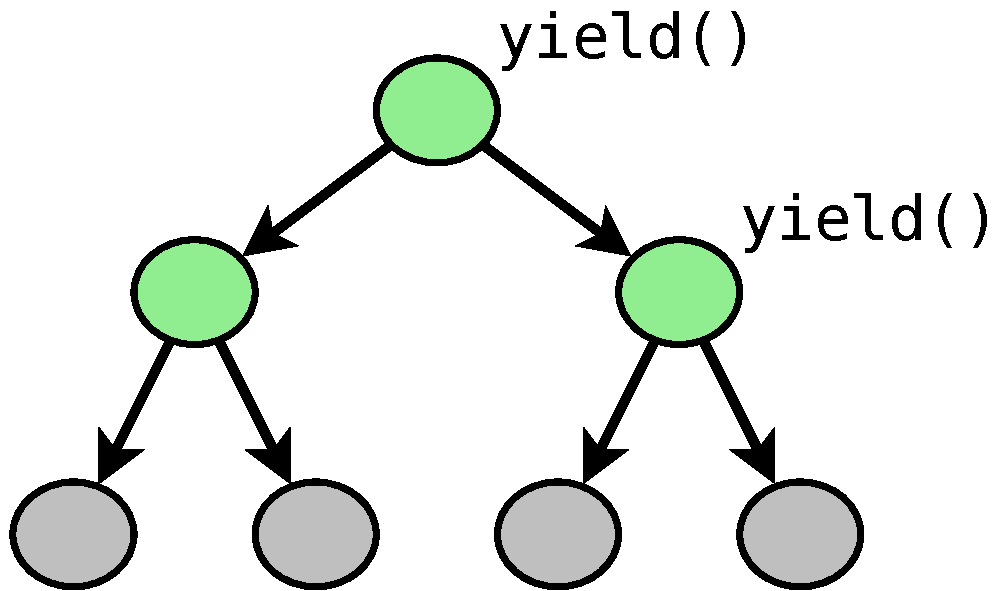
\includegraphics[width=0.35\textwidth]{tree0.pdf}
	\end{center}
\end{frame}

\begin{frame}{Iterative Deepening}
	Adding different PPs can produce state spaces of different sizes; Landslide tries them in parallel.
	\vspace{0.15in}
	\begin{center}
		\begin{tabular}{cc}
			\includegraphics[width=0.45\textwidth]{tree1.pdf} &
			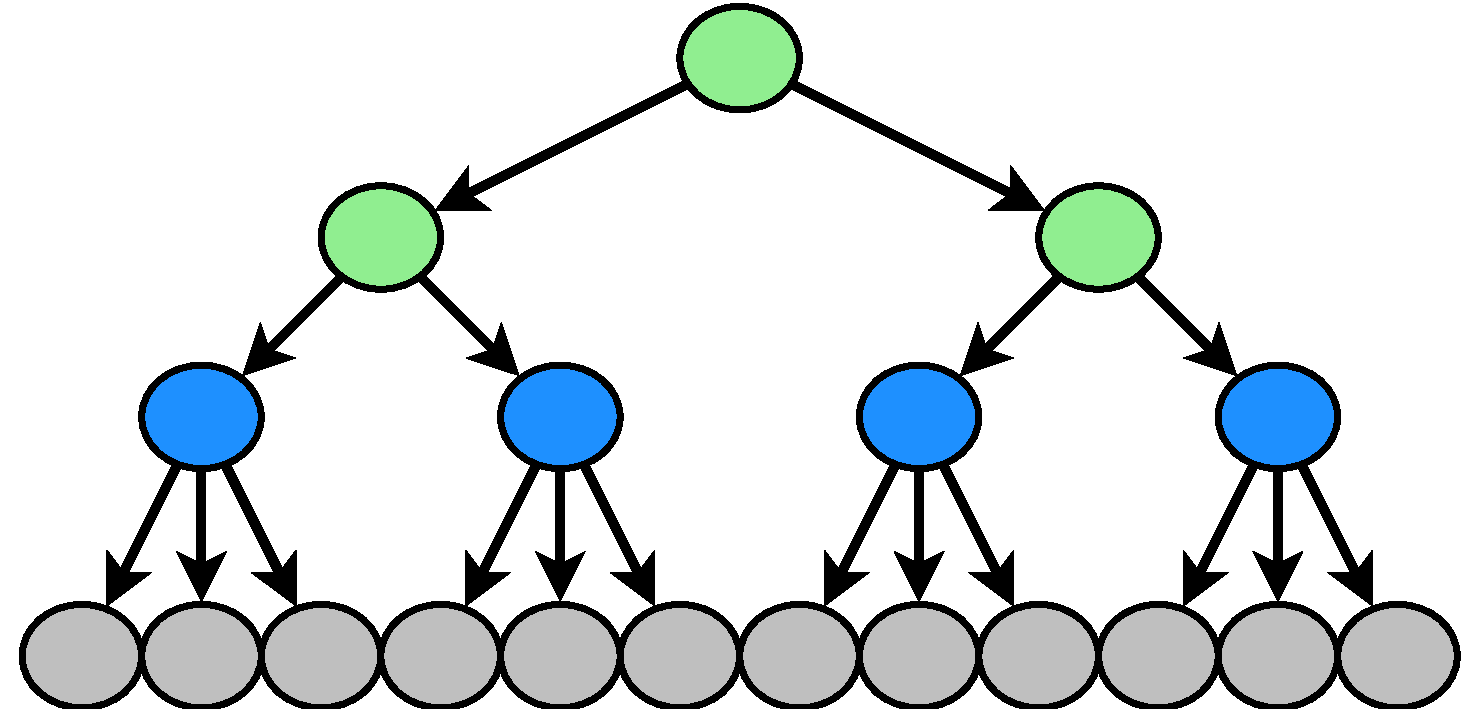
\includegraphics[width=0.5\textwidth]{tree2.pdf}
		\end{tabular}
	\end{center}
\end{frame}


\begin{frame}{Iterative Deepening}
	If time allows, Landslide will combine PPs into larger, more comprehensive state spaces.
	\begin{center}
		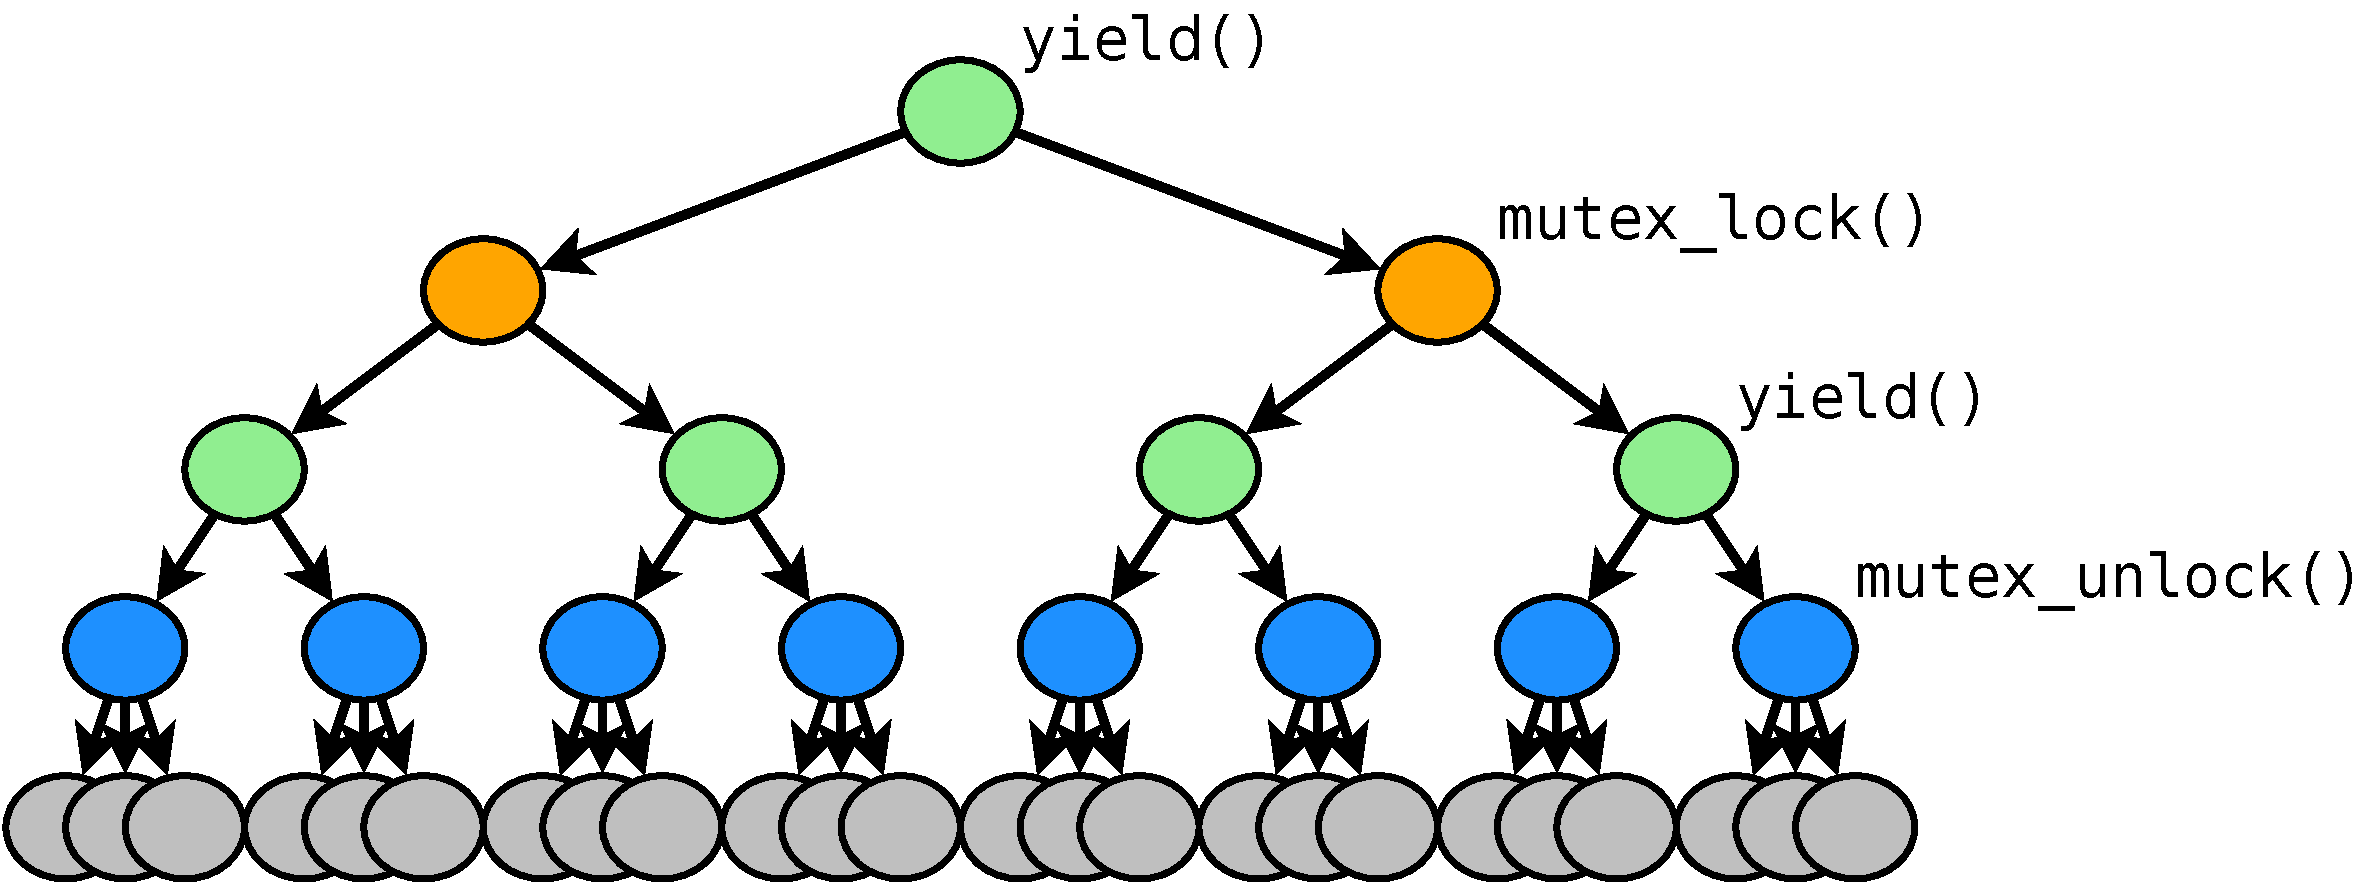
\includegraphics[width=0.8\textwidth]{tree3.pdf}
	\end{center}
	% say: and depending on your time budget, you might decide that you expect this one to be feasible, or you might fall back to a smaller state space from before.
\end{frame}

%%%%%%%%%%%%%%%%%%%%%%%%%%%%%%%%%%%%%%%%%%%%%%%%%%%%%%%%%%%%%%%%%%%%%%%%%%%%%%%%
%%%%%%%%%%%%%%%%%%%%%%%%%%%%%%%%%%%%%%%%%%%%%%%%%%%%%%%%%%%%%%%%%%%%%%%%%%%%%%%%
%%%%%%%%%%%%%%%%%%%%%%%%%%%%%%%%%%%%%%%%%%%%%%%%%%%%%%%%%%%%%%%%%%%%%%%%%%%%%%%%

\section{Evaluation}

\breakslide{\Huge Demo}

\begin{frame}{Test Suite}
	Landslide ships with 6 approved test cases:
	\linegap

	Standard P2 tests
	\begin{itemize}
		\item {\tt thr\_exit\_join}
		\item {\tt paraguay}
		\item {\tt rwlock\_downgrade\_read\_test}
	\end{itemize}

	New tests
	\begin{itemize}
		\item {\tt broadcast\_test}
		\item {\tt paradise\_lost} %(new this semester)
		\item {\tt mutex\_test} %(new this semester)
	\end{itemize}
\end{frame}

%\begin{frame}{Preliminary Evaluation}
%	We tested 22 random submitted P2s from Spring 2014.
%	\begin{itemize}
%		\item Test cases:
%		\begin{itemize}
%			\item {\tt thr\_exit\_join}
%			\item {\tt paraguay}
%			\item {\tt rwlock\_downgrade\_read\_test}
%			\item {\tt broadcast\_test} (new)
%		\end{itemize}
%		\item Each test given CPU budget of 11 cores $\times$ 10 minutes.
%	\end{itemize}
%\end{frame}
%
%\begin{frame}{Preliminary Results}
%%	88 total tests were run (9,680 total CPU-minutes)
%%	\linegap
%%
%	Found 7 {\bf deterministic} initialization bugs (e.g. use-after-free)
%	\linegap
%
%	56 tests ran to completion without finding bugs:
%	\begin{itemize}
%		\item 47 exhausted the CPU budget.
%		\item 9 completed all state spaces before time ran out.
%	\end{itemize}
%	\linegap
%
%	Between 20 and 33 {\bf non-deterministic} bugs were found:
%	\begin{itemize}
%		\item 20 deadlock races among 12 P2s
%		\item 10 use-after-free races among 6 P2s
%		\item 3 misc (assert fail, segfault) among 2 P2s
%	\end{itemize}
%\end{frame}

\begin{frame}{Last Semester}
	%Spring 2015: 7 groups signed up to use Landslide; 5 found bugs
	%%\begin{itemize}
	%%	\item (that they didn't find during stress testing)
	%%\end{itemize}
	%%%%% hopefully!
	%\linegap

	%Among all groups, 38 total tests were run
	%\begin{itemize}
	%	\item 21 tests ran to completion without finding bugs
	%	\item 4 {\em deterministic} bugs
	%	\item 13 distinct {\em non-deterministic} bugs
	%		\begin{itemize}
	%			\item 6 in {\tt thr\_exit\_join} \small (use-after-free, deadlock, NULL, infinite loop...)
	%			\item 4 in {\tt paraguay} (deadlock, infinite loop)
	%			\item 2 in {\tt broadcast\_test} (deadlock, infinite loop)
	%			\item 1 in {\tt rwlock\_downgrade\_read\_test} (use-after-free)
	%		\end{itemize}
	%		%\begin{itemize}
	%		%	\item 6 of which required data-race PPs to expose
	%		%\end{itemize}
	%\end{itemize}
	Fall 2015: 22 groups signed up to use Landslide; 21 found bugs
	% 18 groups found races
	\begin{itemize}
		\item (that they didn't find during stress testing)
	\end{itemize}
	%%%% hopefully!
	\linegap

	Among all groups, 185 distinct tests were run
	\begin{itemize}
		\item 137 tests ran to completion without finding bugs
		\item 21 {\em deterministic} bugs
	\end{itemize}
	\pause % ask: "who can tell me why landslide might find a *deterministic* bug not found during past testing? A: use-after-free
	\linegap

	38 distinct {\em non-deterministic} bugs
	\begin{itemize}
			%\begin{itemize}
			%	\item 7 of which required data-race PPs to expose
			%\end{itemize}
		\item 11 groups (50\%) fixed all their bugs
			\begin{itemize}
				\item (as verified by running Landslide again -- not a guarantee!)
			\end{itemize}
		\item 2.7 bugs ``fixed'' (see above) on average per group
		\item Most ambitious group: 11 distinct races found + fixed!
	\end{itemize}
\end{frame}

%\begin{frame}{A new treat} %since last semester}
%	\texttt{mutex\_test} tries to make your mutexes fail or deadlock.
%	\linegap
%
%	Landslide will look for data races inside your mutex implementation.
%	\begin{itemize}
%		\item {\tt xchg}/{\tt cmpxchg}/{\tt xadd}
%		\item {\tt mutex->whose\_turn\_is\_it = ...;}
%	\end{itemize}
%	\pause
%	\linegap
%	
%	Last semester: 12 non-determinstic bugs among 8 groups
%	\linegap
%
%	%Tested 77 P2s from S'14, F'14, S'15
%	%\begin{itemize}
%	%	\item 5 unrelated deterministic bugs (use-after-free, crash, etc)
%	%		% TODO check these for false positives
%	%		% But this was run after the arbiter fp deadlock avoidance
%	%		% So I think it's ok
%	%	\item 7 deadlock races
%	%	\item 4 other races (NULL crash, infinite loop, use-after-free)
%	%	\item 1 ``two threads got the lock at once'' race
%	%		\begin{itemize}
%	%			\item {\em ...that the TA who graded it didn't find!}
%	%		\end{itemize}
%	%\end{itemize}
%\end{frame}


%%%%%%%%%%%%%%%%%%%%%%%%%%%%%%%%%%%%%%%%%%%%%%%%%%%%%%%%%%%%%%%%%%%%%%%%%%%%%%%%

\subsection{Landslide for the People}

\begin{frame}{User Study}
	\textbf{Try Landslide on your P2!}
	\begin{itemize}
		\item Bare minimum effort: No more than 1 hour
		\begin{itemize}
			\item Clone a github URL, run setup script, run tests %, answer survey questions
			\item Landslide will automatically report test results
		\end{itemize}
		\item Full study plan: 4-8 hours of active attention
		\begin{itemize}
			\item (Estimated, including time to diagnose and fix bugs)
			\item However, many tests should run passively overnight -- start soon!
		\end{itemize}
	\end{itemize}
	\pause
	\linegap

	Prerequisites
	\begin{itemize}
		\item You {\em must} pass the P2 hurdle before using Landslide.
		\begin{itemize}
			\item {\tt startle}, {\tt agility\_drill}, {\tt cyclone}, {\tt join\_specific\_test}, {\tt thr\_exit\_join}
		\end{itemize}
		\item Must have {\em attempted} several stress tests
		\begin{itemize}
			\item {\tt juggle 4 3 2 0}, {\tt multitest}, {\tt racer} (15 min), {\tt paraguay}
		\end{itemize}

	\end{itemize}
\end{frame}

\begin{frame}{User Study - Additional Information}
	Human Subjects Research
	\begin{itemize}
		\item CMU IRB has approved this study
		\item Landslide will collect results while you use it
		\begin{itemize}
			\item Record commands issued, take snapshots of your P2 code
			\item All data will be anonymized before publication
		\end{itemize}
		\item No coercion: {\bf \em There is no penalty for not participating.}
		\begin{itemize}
			\item I am not on course staff, cannot influence your grade
			\item Course staff will not have access to study data during semester
		\end{itemize}
	\end{itemize}
	\pause
	\linegap

	Risks \& Benefits
	\begin{itemize}
		\item Benefit: Landslide may help you find/fix bugs, improving your grade!
		\item Risk: Landslide may find no bugs and be a waste of your time.
		\item Benefit: You might learn something...
	\end{itemize}
	% Say: Accordingly, although I hope you will use landslide enough to get good results for me, you should also responsibly allocate time between testing with landslide versus actually implementing your P2.
\end{frame}

\begin{frame}{User Study - How to Participate}
	Interested?
	\linegap

	To participate\dots
	\begin{itemize}
		\item Review this lecture and study information sheet
		\item Meet prerequisites of passing P2 tests
		\item Complete sign-up form online to get further instructions
			\begin{itemize}
				\item \url{http://tinyurl.com/landslide-p2-s16}
			\end{itemize}

		\item Use Landslide in addition to stress tests until P2 is due!
	\end{itemize}
	\linegap

	{\em Really} interested?
	\begin{itemize}
		\item I know of an M.S. thesis topic if you want to do post-OS research.
	\end{itemize}
\end{frame}

%%%%%%%%%%%%%%%%%%%%%%%%%%%%%%%%%%%%%%%%%%%%%%%%%%%%%%%%%%%%%%%%%%%%%%%%%%%%%%%%
%%%%%%%%%%%%%%%%%%%%%%%%%%%%%%%%%%%%%%%%%%%%%%%%%%%%%%%%%%%%%%%%%%%%%%%%%%%%%%%%
%%%%%%%%%%%%%%%%%%%%%%%%%%%%%%%%%%%%%%%%%%%%%%%%%%%%%%%%%%%%%%%%%%%%%%%%%%%%%%%%

\section{End}
\breakslide{\Large Questions?
\linegap

\begin{center}
	\includegraphics[width=0.65\textwidth]{3word-questions.png}
\end{center}}

%%%%%%%%%%%%%%%%%%%%%%%%%%%%%%%%%%%%%%%%%%%%%%%%%%%%%%%%%%%%%%%%%%%%%%%%%%%%%%%%
%%%%%%%%%%%%%%%%%%%%%%%%%%%%%%%%%%%%%%%%%%%%%%%%%%%%%%%%%%%%%%%%%%%%%%%%%%%%%%%%
%%%%%%%%%%%%%%%%%%%%%%%%%%%%%%%%%%%%%%%%%%%%%%%%%%%%%%%%%%%%%%%%%%%%%%%%%%%%%%%%

\section{Bonus Slides}

%\subsection{Experimental Results}
%
%\begin{frame}{More Evaluation}
%	\textbf{Is dynamically adding ``data race'' PPs effective?}
%	\begin{itemize}
%		%\item 3 among preliminary bugs (9-15\%) required data races to expose.
%		\item 6 among S'15 student bugs (46\%)
%		\item 10 among {\tt mutex\_test} bugs (71\%)
%	\end{itemize}
%	\linegap
%
%	{\bf Is ``iterative deepening'' better than state-of-the-art?}
%	\begin{itemize}
%		\item Control experiment: Just 1 state space, same CPU time
%		\begin{itemize}
%			\item PPs used: \texttt{mutex\_lock()}, \texttt{mutex\_unlock()}
%			\item 110 minutes on 1 CPU
%		\end{itemize}
%		\item Of 33 total bug reports, control failed to find 10 (30\%).
%		\begin{itemize}
%			\item 3 required data race PPs to expose
%			\item 1 ran out of time
%			\item 6 obscured by different bug in same state space
%		\end{itemize}
%	\end{itemize}
%\end{frame}

\begin{frame}{Last-last Semester}
	Spring 2015: 7 groups signed up to use Landslide; 5 found bugs
	%\begin{itemize}
	%	\item (that they didn't find during stress testing)
	%\end{itemize}
	%%%% hopefully!
	\linegap

	Among all groups, 38 total tests were run
	\begin{itemize}
		\item 21 tests ran to completion without finding bugs
		\item 4 {\em deterministic} bugs
		\item 13 distinct {\em non-deterministic} bugs
			\begin{itemize}
				\item 6 in {\tt thr\_exit\_join} \small (use-after-free, deadlock, NULL, infinite loop...)
				\item 4 in {\tt paraguay} (deadlock, infinite loop)
				\item 2 in {\tt broadcast\_test} (deadlock, infinite loop)
				\item 1 in {\tt rwlock\_downgrade\_read\_test} (use-after-free)
			\end{itemize}
			%\begin{itemize}
			%	\item 6 of which required data-race PPs to expose
			%\end{itemize}
	\end{itemize}
\end{frame}

\subsection{State Space Reduction}

\begin{frame}{Coping with State Space Explosion}
	Serious problem: State spaces grow exponentially
	\begin{itemize}
		\item With $p$ preemption points and $k$ runnable threads, size $p^k$.
		\item Threatens our ability to explore everything.
		\item Fortunately, some sequences result in identical states.
	\end{itemize}
	\linegap

	{\bf Partial Order Reduction} identifies and skips ``equivalent'' interleavings.
	\begin{itemize}
		\item After each execution, compare memory reads/writes of each thread.
		\item Find when reordering threads couldn't possibly change behaviour.
		\item Example follows\dots
	\end{itemize}
\end{frame}

\begin{frame}{State Space Reduction}
	\begin{center}
	\includegraphics[width=\textwidth]{undiamond0.png}
	\end{center}
\end{frame}
\begin{frame}{State Space Reduction}
	\begin{center}
	\includegraphics[width=\textwidth]{undiamond1.png}
	\end{center}
\end{frame}
\begin{frame}{State Space Reduction}
	\begin{center}
	\includegraphics[width=\textwidth]{diamond1.png}
	\end{center}
\end{frame}

\end{document}
